% !TEX root = ../Thesis.tex

\chapter{Sistemi Operativi}\label{cap:04}

Questo capitolo esplorerà le capacità offerte da Rust nel 
contesto della programmazione di sistema. In apertura verrà
fornita una panoramica sul linguaggio C, standard \textit{de facto}
nel contesto programmazione di sistema, con particolare attenzione alle 
 caratteristiche che lo rendono popolare in questo ambito.

Successivamente Rust verrà confrontato con C rispetto agli aspetti analizzati
, per valutare come Rust possa presentare un'alternativa valida sul piano teorico.

Nel capitolo~\ref{cap:05}, `\textit{<inserire nome>}', l'analisi verrà spostata sul piano pratico, 
esplorando progetti concreti, che mostrano le potenzialità di Rust nella programmazione di basso livello. \hfill
\vspace{20pt}\\
\noindent Nel contesto dei sistemi operativi, quali lo sviluppo di kernel, driver o componenti embedded i linguaggi tradizionalmente dominanti
 sono l'assembly e, con maggiore rilievo, C.

Nonostante l'esistenza di alternative come C++, Lisp, Forth o Bliss, la scelta spesso ricave esclusivamente
su C, come testimoniano le codebase dei sistemi operativi più popolari oggi giorno: Windows, MacOS, Linux e Android sono scritti quasi interamente nel linguaggio C.

Ma cosa rende C così popolare in questo ambito? Quali caratteristiche lo distinguono dalle alternative?

\section{C:\  motivazioni e caratteristiche}
C è un linguaggio di programmazione ampiamente utilizzato nella 
programmazione di sistema. Il linguaggio offre un livello
di astrazione molto vicino al codice macchina (o meglio, 
all'assembly), garantendo un certo grado di portabilità 
tra architetture differenti.

Si consideri, per esempio, quanto detto dal creatore del linguaggio:
\begin{center}
    \begin{minipage}{0.9\textwidth}
        \vspace{0.5em}
        \itshape "[C has] the power of the assembly language and the convenience of \ldots assembly language."

        \hfill --- Dennis Ritchie, creatore del linguaggio C, "Dennis Ritchie: The Shoulders Steve Jobs Stood On", *Wired*, 13 Oct 2011
        \vspace{0.4em}
    \end{minipage}
\end{center}
\noindent La popolarità di C in questo ambito è da attribuire a
diverse sue caratteristiche, alcune delle quali ben documentate\cite{c-system-programming-why}. 
Queste sono principalmente: compilazione, assenza di dipendenze 
runtime, gestione diretta della memoria, manipolazione 
a basso livello di bit e corrispondenza quasi diretta al codice macchina.

\subsection*{Compilazione}
C è un linguaggio compilato: il file eseguibile generato risulta 
molto efficiente, sotto l'aspetto della velocità d'esecuzione, 
rispetto a linguaggi interpretati. Questo lo rende preferibile nell'ambito di sviluppo
kernel, dove le prestazioni rappresentano un aspetto cruciale.

\subsection*{Assenza di dipendenze runtime}
C può essere impiegato per realizzare codice 
`\textit{bare metal}', eseguibile direttamente sull'hardware, 
senza il supporto di un sistema operativo. 

C non ha esigenze runtime significative: può funzionare anche senza un allocatore di memoria fornito dal 
sistema operativo\footnote{Un programma che non usufruisce della memoria 
dinamica non richiede un allocatore. Inoltre, nello sviluppo di un sistema 
operativo, è il programmatore che deve fornire il proprio sistema di allocazione.}. L'unica 
necessità minima è quella di un chiamante che invochi la funzione \textit{main}\footnote{In contesti a basso livello, quest a chiamata 
 può essere realizzata da codice assembly.}.

\subsection*{Accesso diretto alla memoria}
I puntatori C consentono l'accesso diretto a
indirizzi di memoria arbitrari, permettendo operazioni di lettura e 
scrittura dirette. 

Tale controllo sulla memoria è cruciale per lo sviluppo di un 
sistema operativo, dove è richiesto di gestire: tabelle delle pagine, dispositivi I/O mappati sulla memoria, controllori DMA e altri;

\subsection*{Manipolazione di bit}
Molte interazioni con l'hardware avvengono tramite operazioni bitwise, come riportato da \textit{Ada Computers}\cite{bitwise-operations}. 
Esempi comuni sono:
\begin{itemize}
    \item Operazioni di scrittura e lettura dei registri della CPU, come registri di flag di stato. Per esempio, in CPU x86 si trova il registro \textit{EFLAGS} che contiene una serie di bit di stato (\textit{overflow}, \textit{zero}, \textit{carry}, \textit{interrupt enable} e altri), il loro controllo di solito è fatto tramite l'applicazione di una maschera bitwise;
    \item Gestione delle periferiche mappate sulla memoria, tramite operazioni di abilitazione e disabilitazione dei singoli pin (e.g.\  registri \textit{GPIO});
    \item Il clock della CPU può essere gestito tramite operazioni bitwise.
\end{itemize}
Come riportato dal seguente articolo~\cite{bitwise-operations-c}, il linguaggio C supporta un ampio range di operazioni bitwise, offrendo i seguenti operatori: \textit{AND}, \textit{OR}, \textit{XOR}, \textit{SHL}, \textit{SHR}, \textit{NOT} e il complemento.

\subsection*{Somiglianza al codice macchina}
C mantiene una corrispondenza quasi \textit{1-to-1} in codice assembly. 
Questa trasparenza del linguaggio è fondamentale nello sviluppo di 
sistemi operativi, in quanto consente di comprendere l'effetto di ogni singola istruzione. 
C evita strutture dati complesse o astrazioni pesanti che potrebbero mascherare
il comportamento a basso livello del programma.\hfill
\vspace{30pt}\\
\noindent Tuttavia, uno dei punti di forza di C rappresenta anche una sua criticità. 
L'accesso diretto e non controllato della memoria, unito all'assenza di protezioni a runtime, rende semplice
commettere errori potenzialmente gravi come:
\begin{itemize}
    \item \textbf{Accessi non autorizzati alla memoria}: un programma che legge da un indirizzo di memoria arbitrario potrebbe inavvertitamente compromettere la privacy di un'altro processo; una scrittura accidentale potrebbe causare la corruzione della memoria, condivisa o utilizzata da un altro processo;
    \item \textbf{Saturazione della memoria}: un programma che alloca memoria senza controllo o limiti potrebbe esaurire la memoria disponibile. Se lo \textit{swapping} è disponibile, il sistema può degradare drasticamente le prestazioni; in caso non lo fosse, può verificarsi un crash.
\end{itemize}

\section{Rust contro C}
Nonostante Rust offra numerose astrazioni di alto livello\footnote{Rust offre delle astrazioni di alto livello definite \textit{zero cost}: feature quali \textit{iteratori}, \textit{generics}, \textit{smart pointers} e meccanismi di \textit{async/await} che vengono compilate in codice dalle prestazioni equivalenti alla controparte \textit{low-level} scritta a mano.}, è progettato come un linguaggio di basso livello, 
adatto alla programmazione di sistema.
Per comprendere le capacità di Rust nella programmazione di basso livello, verrà confrontato con il linguaggio C, sulla 
base delle caratteristiche che lo rendono favorevole nella programmazione di sistema.

La maggior parte delle informazioni riportate nella sezione è stata ricavata dalla documentazione ufficiale di Rust\cite{rust-book}.
\begin{itemize}
    \item \textbf{Compilazione} (Come C): Anche Rust è un linguaggio compilato. Il compilatore genera, in base alla piattaforma, un file direttamente eseguibile;
    \item \textbf{Dipendenze runtime} (Come C): Rust, per configurazione predefinita, ha dipendenze runtime minime (principalmente un allocatore di memoria). Tuttavia, come riportato in \textit{The Embedded Rust Book}\cite{rust-book-embedded}, tramite la direttiva \texttt{\#![no\_std]} è possibile escludere la libreria standard: in questa configurazione, l'unico requisito è un bootstrap che invochi la funzione \texttt{\_start} per fare iniziare l'esecuzione;
    \item \textbf{Accesso diretto alla memoria} (Come C): Tramite una parola chiave, \textit{unsafe}, Rust mette a disposizione cinque operazioni denominate \textit{superpoteri non sicuri}: tra queste si trovano anche la possibilità di dereferenziare un puntatore raw (come in C) e la possiblità di eseguire codice C o assembly;
    \item \textbf{Manipolazione di bit} (Come C): Rust offre lo stesso livello di manipolazione dei singoli bit di C, con un'unica differenza: le operazioni bitwise in Rust sono ben definite, evitando condizioni di \textit{Undefined Behaviour} tramite controlli statici sulle dimensione e tipi degli operandi;
    \item \textbf{Somiglianza al codice macchina} (Diverso da C): Rust generalmente offre astrazioni di alto livello, inoltre il compilatore può introdurre copie e spostamenti aggiuntivi per preservare le condizioni di ownership o inserire controlli su accessi e indici per gli \textit{slice}\footnote{Slice è un tipo primitivo in Rust. Sono un riferimento a una porzione contigua (in memoria) di elementi di una collezione. Non memorizzano dati esplicitamente, si tratta di una vista su dati esistenti.}. Tali comportamenti, pur aumentando la sicurezza, possono produrre un codice meno `trasparente' rispetto alla controparte C;\ 
\end{itemize}
Infine, a differenza di C, Rust garantisce l'integrità e la sicurezza della memoria già a tempo della compilazione, prevenendo 
errori comuni legati alla gestione della memoria grazie al \textit{modello di ownership}. In quanto i controlli effettuati
dal \textit{Borrow Checker} avvengono a tempo di compilazione non si hanno dipendenze o overhead introdotti a runtime.

\subsection*{Unsafe Rust}
Come già accennato, Rust mette a disposizione, tramite la parola chiave \textit{unsafe}, cinque operazioni principali. Gli sviluppatori
del progetto Rust si riferiscono a queste operazioni con l'espressione \textit{Unsafe Superpowers}:
\begin{itemize}
    \item Dereference di un puntatore raw;
    \item Invocazione di una funzione o metodo non sicuri;
    \item Accesso e modifica di una variabile mutabile e statica;
    \item Implementazione di un tratto non sicuro;
    \item Accesso ai campi di una \textit{union}.
\end{itemize}
Le espressioni \textit{Unsafe Rust} e \textit{Unsafe Superpowers} possono risultare fuorvianti: il \textit{Borrow Checker} esegue 
comunque controlli per garantire la validità delle reference. 

La parola chiave permette solamente di eseguire operazioni che, per definizione, sono considerate non sicure. 
Il compilatore non può controllarne la sicurezza e l'integrità durante la compilazione; all'interno di un blocco
 \textit{unsafe}, è il programmatore a diventare responsabile di garantire che gli accessi alla memoria
siano validi. \hfill
\vspace{12pt}\\
\noindent La \textit{best practice} riguardante i blocchi non sicuri prevede di ridurre il codice non sicuro il più possibile, utilizzandolo solo quando stretto necessario.
Inoltre, è preferito incapsulare il codice non sicuro all'interno di un'astrazione sicura, fornendo una API sicura per il suo utilizzo. \hfill
\subsection{Gestione delle risorse}
\subsection{Sicurezza della memoria}
In questa sottosezione verranno analizzati alcuni tra gli errori più comuni legati alla gestione della memoria,
mostrando esempi di codice scritti in C e confrontandoli, quando possibile, con le controparti in Rust.

Un aspetto interessante del modello di memoria di Rust è che alcuni errori non sono semplicemente rilevati
durante l'esecuzione, o a tempo di compilazione, ma sono strutturalmente impossibili da generare.
Come già accennato, il \textit{modello di ownership} guida la struttura di un programma in Rust: spinge il programmatore a
ragionare in termini di \textit{ownership} e \textit{lifetime}.
Come conseguenza diretta, alcuni problemi frequenti come \textit{dangling pointers}, \textit{double free} o \textit{use after free} sono
impediti staticamente: il compilatore rifiuta di compilare codice che potenzialmente potrebbe causarli.

\subsubsection{Memoria non liberata (\textit{unfreed memory})}
La memoria non liberata rappresenta un errore comune durante la gestione della memoria dinamica tramite approccio manuale.
Si ha in quei contesti in cui la memoria viene allocata, senza venire deallocata esplicitamente. Queste aree di memoria non
possono essere riutilizzate per allocazioni successive in quanto vengono considerate ancora utilizzate.
Si consideri il seguente esempio minimale C che genera un'errore di unfreed memory:
\begin{lstlisting}[language=C, caption={Unfreed memory in C}, label={c:unfreed-memory}]
#include <stdlib.h>
int main(void) {
    void* mem = malloc(sizeof(int));
    return 0;
}
\end{lstlisting}
In Rust questo comportamento non si potrà mai realizzare, in quanto la deallocazione viene gestita implicitamente dal compilatore\footnote{Il compilatore inserisce chiamate alla funzione \textit{drop} in corrispondenza della fine di uno scope. Questo è realizzabile in quanto il \textit{Borrow Checker} controlla le relazioni di \textit{ownership} e \textit{borrowing} per determinare chi sia responsabile della deallocazione, ovvero su quali variabili invocare \textit{drop}.}.
Si consideri un programma in Rust che replica il comportamento del listato precedente:
\begin{lstlisting}[language=Rust, caption={Unfreed memory in Rust}, label={rust:unfreed-memory}]
fn main() {
    let mem = Box::<u32>::new(0);
}
\end{lstlisting}
Nel listato~\ref{c:unfreed-memory} viene allocata memoria nella heap sufficiente a contenere un intero, successivamente 
il programma termina senza liberarla. Il programma viene compilato ed eseguito correttamente, 
nonostante la presenza di questo errore. 

In realtà l'allocazione avviene nello spazio di memoria virtuale del processo; a termine dell'esecuzione, il sistema operativo recupera tutte le risorse allocate dal processo. 
Tuttavia, tale memoria risulta inaccessibile per ulteriori allocazioni da parte del processo durante la sua esecuzione.\hfill
\vspace{10pt}\\
\noindent Il listato~\ref{rust:unfreed-memory} rappresenta il codice Rust più vicino possibile a 
quello del listato precedente. La differenza principale è che la memoria viene deallocata automaticamente: 
al termine dello scope della funzione \texttt{main}, la variabile \texttt{mem} viene eliminata e la relativa 
memoria deallocata. 

Di conseguenza, l'errore di \textit{unfreed memory} non può manifestarsi, in quanto la deallocazione avviene in maniera 
trasparente agli occhi del programmatore. 


% Double free
\subsubsection{Doppia liberazione (\textit{double free})}
La doppia liberazione è un'errore di gestione della memoria che si verifica la stessa area di memoria viene deallocata
più di una volta. Ciò può causare la corruzione della memoria heap, con conseguente comportamento indefinito, crash del programma o
potenziali vulnerabilità di sicurezza.

Nel linguaggio C, questo si verifica invocando la funzione \texttt{free} sullo stesso puntatore più volte, come mostrato 
nel seguente esempio:
\begin{lstlisting}[language=C, caption={Double free in C}, label={c:double-free}]
#include <stdlib.h>
int main(void) {
    void* mem = malloc(sizeof(int));
    free(mem);
    free(mem);
    return 0;
}
\end{lstlisting}
Si consideri invece il seguente programma Rust che tenta di replicare lo stesso comportamento del listato~\ref{c:double-free}:
\begin{lstlisting}[language=Rust, caption={Double free in Rust}, label={rust:double-free}]
fn main() {
    let mem = Box::<u32>::new(0);
    std::mem::drop(mem);
    std::mem::drop(mem);
}
\end{lstlisting}
Nel listato~\ref{c:double-free} la memoria puntata da \texttt{mem} viene deallocata due volte.
In fase di esecuzione questo può portare a un crash del programma, come mostrato nell'immagine~\ref{c:double-free-exec}.

Tuttavia, lo standard C non definisce un comportamento specifico da adottare in questo contesto, causando 
\textit{undefined behaviour} nella pratica\footnote{In ambiente Linux con \texttt{glibc}, viene rilevato l'errore causando
 la stampa di un messaggio e l'interruzione dell'esecuzione. In ambienti Windows, l'errore può passare inosservato o causare un crash silenzioso.}.

Per quanto riguarda Rust, è possibile considerare due scenari: 
\begin{itemize}
    \item Il listato~\ref{rust:unfreed-memory} rappresenta il comportamento idiomatico di Rust: la memoria viene deallocata automaticamente alla fine di uno \textit{scope}, senza necessità di interventi manuali;
    \item Nel listato~\ref{rust:double-free}, invece, si tenta di deallocare esplicitamente la memoria con due chiamate consecutive a \texttt{std::mem::drop}\footnote{Questa funzione causa uno spostamento dell'\textit{ownership} del valore fornito, causandone la deallocazione una volta raggiunta la fine dello scope.}. Tuttavia, la funzione \texttt{drop} prende possesso del valore, rendendo la reference originale, e di conseguenza la seconda chiamata, invalida. Il compilatore si accorge della violazione della terza regola di \textit{borrowing (Tutte le reference devono essere valide)}, impedendo la compilazione e generando l'errore riportato nell'immagine~\ref{rust:double-free-compile}.
\end{itemize}
\begin{figure}[htbp]
\begin{center}
    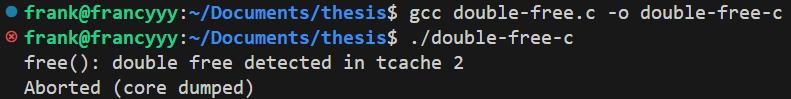
\includegraphics[width=.8\textwidth]{double-free-c-exec}
    \caption{\textit{Double free} in C}\label{c:double-free-exec}
    \end{center}
\end{figure}
\begin{figure}[htbp]
\begin{center}
    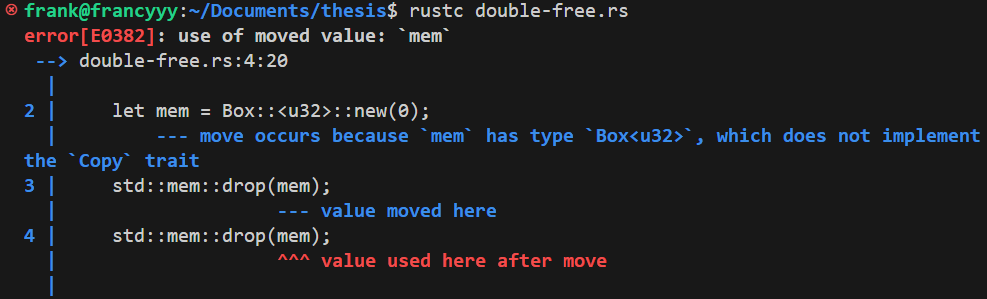
\includegraphics[width=.8\textwidth]{double-free-rust-compile}
    \caption{Tentativo di \textit{double free} in Rust}\label{rust:double-free-compile}
    \end{center}
\end{figure}

% Dangling pointer e Access after free
\subsubsection{Puntatori pendenti (\textit{dangling pointers})}
Un \textit{dangling pointer} è un puntatore che continua a riferire a una locazione di memoria non più valida o che è stata liberata. 
Generalmente accade quando un'area di memoria viene deallocata, ma eventuali puntatori che la referenziavano non vengono aggiornati correttamente.
Si consideri il seguente esempio C che genera un \textit{dangling pointer}:
\begin{lstlisting}[language=C, caption={Dangling pointer in C}, label={c:dangling-pointer}]
int main(void) {
    int* ptr;
    {
        int* val = malloc(sizeof(int));
        *val = 30;
        ptr = val;
        free(val);
    }
}
\end{lstlisting}
Nel listato~\ref{c:dangling-pointer}, viene allocata memoria sufficiente per un intero e il suo indirizzo è memorizzato 
sia in \texttt{val} che in \texttt{ptr}. La memoria viene successivamente deallocata invocando la funzione free sul puntatore val.
Tuttavia, il puntatore ptr non viene aggiornato, facendo riferimento a memoria non più valida.

è opportuno osservare che la sola esistenza un un dangling pointer non genera un errore immediato.
Si può presentare un comportamento indefinito solo quando si tenta di derefenziarlo, per leggerne o modificarne il contenuto.


Anche in Rust si riflette questa considerazione, è possibile creare una dangling reference, a patto che non venga usata, come mostrato dal seguente esempio
\begin{lstlisting}[language=Rust, caption={Dangling reference in Rust}, label={rust:dangling-pointer}]
fn main() {
    let _ref: &u32;
    {
        let val = Box::<u32>::new(30);
        _ref = &*val;
    }
}
\end{lstlisting}
Il listato~\ref{rust:dangling-pointer} tenta di emulare il comportamento descritto nel listato precedente~\ref{c:dangling-pointer}. è interessante osservare
che il compilatore accetta questo codice, non generando errori. Questo è dovuto al fatto che la reference non è utilizzata, non generando quindi una criticità
dal punto di vista della sicurezza di memoria: il Borrow Checker infatti, controlla la reference in maniera lazy\footnote{}.

% Access after free
\subsubsection{Accesso post-liberazione (\textit{access after free})}


% Buffer Overflow
\subsubsection{Sovraccarico del buffer (\textit{buffer Overflow})}

% Unitialized memory access
\subsubsection{Accesso a memoria non inizializzata (\textit{unitialized memory access})}

\subsection{Prestazioni}
\subsection{Complessità del codice}
